\documentclass{article}
\title{\huge\textbf{Article On\\COEP Technological University Pune}}
\date{\huge 2022-7-11}
\author{\huge By Nachiket Deshmukh}

\usepackage{graphicx}
\begin{document}
\maketitle
\pagenumbering{Roman}
\newpage
\pagenumbering{arabic}

\tableofcontents
\newpage


\textbf{COEP Technological University}, is A Unitary Public University of Government of Maharashtra ,situated in Pune, Maharashtra, India. Established in 1854, it is the 2nd oldest engineering college in India, after IIT Roorkee (1847).The students and alumni are colloquially referred to as COEPians.On 23 June 2022, \textbf{Government of Maharashtra} issued a notification regarding conversion of college into Unitary Maharashtra Technological university. On 24 March 2022, both the houses of the state government passed the CoEP Technological University bill, which has conferred a unitary state university status on the institute.

\begin{center}
  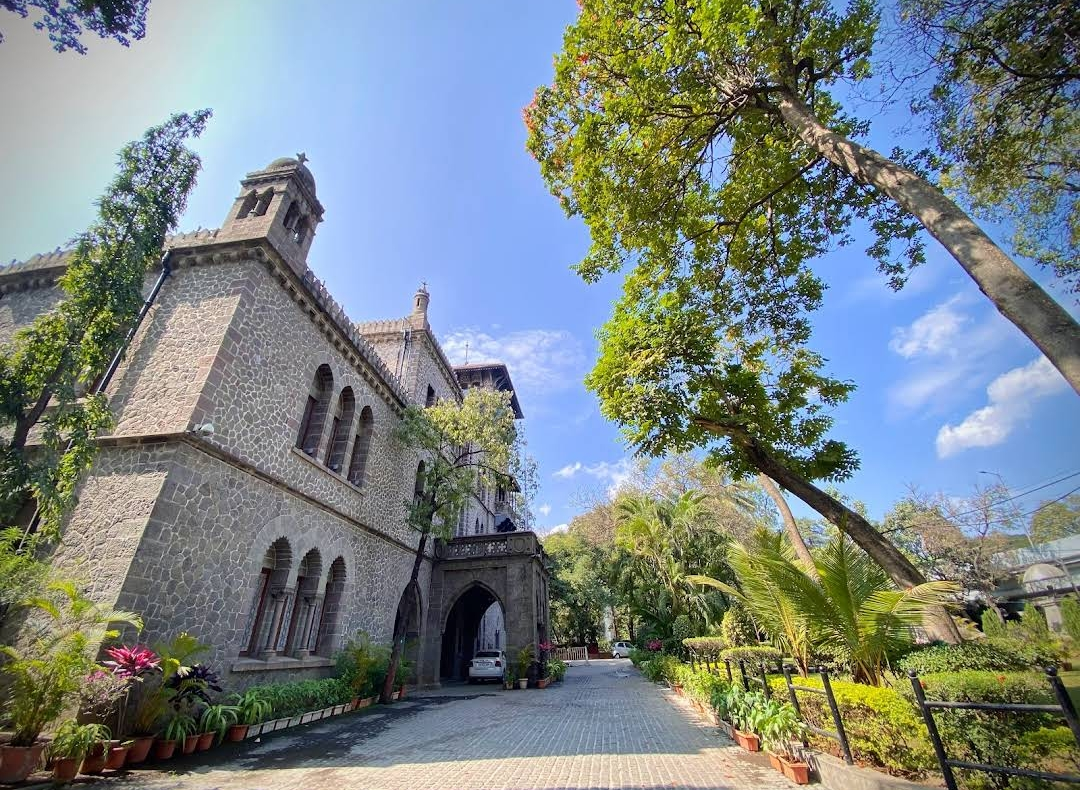
\includegraphics[width=0.7\linewidth]{coep.jpg}
  \label{fig:1} 
\end{center}
\section{History}
The institution was started on \textbf{July 1854}, as the "Poona Engineering and Mechanical School", to train public works department (PWD) officials and was housed in Bhawanipeth, Poona in three houses for teaching purpose and a sepearate house for principal to train subordinate officers in the Public Works Department.In July 1857, Henry Coke was given the charge of the institute. Admission was open to all, irrespective of nationality or caste.Good proficiency in English and basic knowledge of Mathematics were a prerequisite for getting admitted to the institute.The process of admission required that the aspiring candidate apply to the nearest government English school, to whom the entrance examination papers were handed over.
\section{Campus}
The campus of COEP is spread over 36 acres. The campus is divided into four parts North Campus, South Campus, Hostel campus and Playground, due to roadways in between.

The main building is the present day administrative building of the College. It houses the Director, the Dean Academic Affairs, the Dean Student Affairs, the Gymkhana, the Examination cell and other various important administrative heads of the college. The building is almost three floors tall with a base floor length of 18 meters and a width of 9 metres. The building was refurbished in 2012.
\begin{center}
  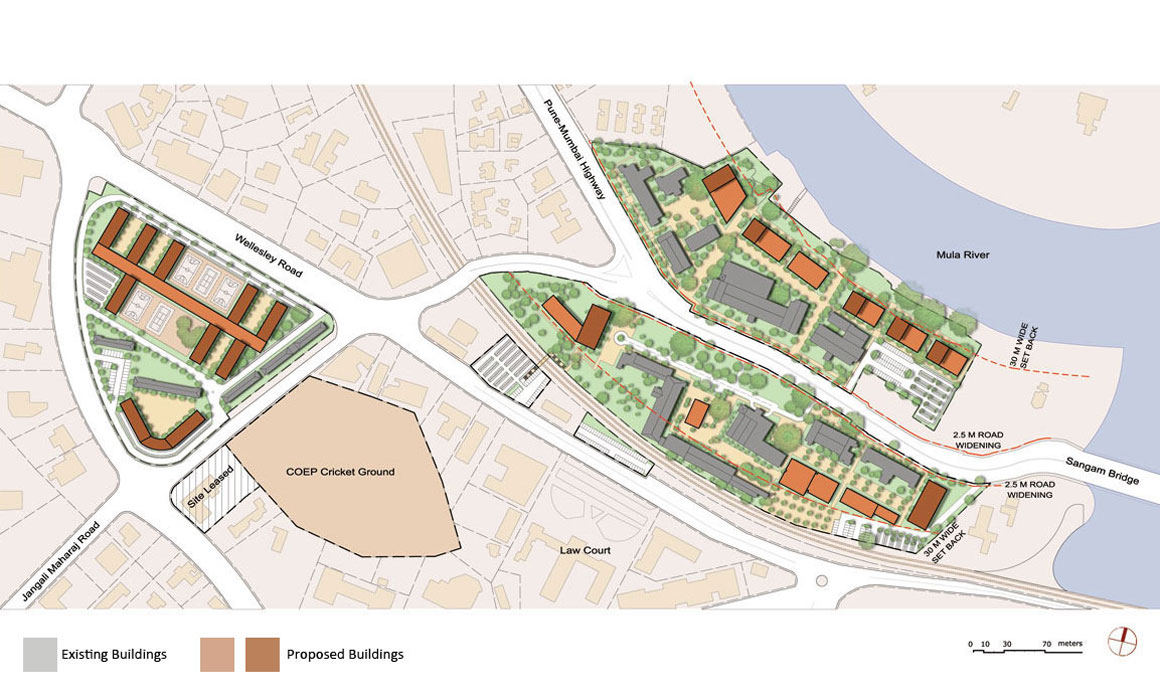
\includegraphics[width=0.7\linewidth]{coep3.jpg}
  \label{fig:2} 
\end{center}
\section{Academics}
\subsection{Admissions}
The admissions are conducted on the basis of the marks secured in Maharashtra CET and HSC board combined. These admissions are conducted by the Directorate of Technical Education (DTE) through the Centralized Admission Process (CAP). Several admissions to direct second year of BTech course are also conducted for those candidates who have completed Diploma in Engineering at different polytechnic institutes in the state of Maharashtra. 

The college also provides Doctor of Philosophy (PhD) programmes in various fields. Department of Applied Sciences is a recognised PhD research centre in the subjects of Environmental Sciences and Chemistry.
\subsection{Rankings}
COEP was ranked 15 among engineering colleges in India by Outlook India in 2019.[24] The National Institutional Ranking Framework (NIRF) ranked it 50th in the engineering ranking in 2020[23] and 101-150 overall.[22] It has been ranked number one among the top five government institutions in Atal Ranking of Institutions on Innovation Achievement (ARIIA) in 2020 and ranked first in 2021
\section{Student Life}
\subsection{Fests}
\subsubsection{Regatta}
Regetta is an annual regatta hosted by the College of Engineering, Pune. Since its inception in 1928, it has showcased around 165 boats, notably the Eighter, which is one of the oldest boats.[28] The 92nd edition of Regatta was held on 8 March 2020. Unlike a Regatta which means a collection of boat races, COEP Boat Club's Regatta is a show of various kinds of boats, kayaks, punts, shell boats and scull boats. The events in this show are Telematches, Kayak Ballet, Shell Games, Punt Formation, Mashaal Dance and the Arrow formation.
\begin{center}
  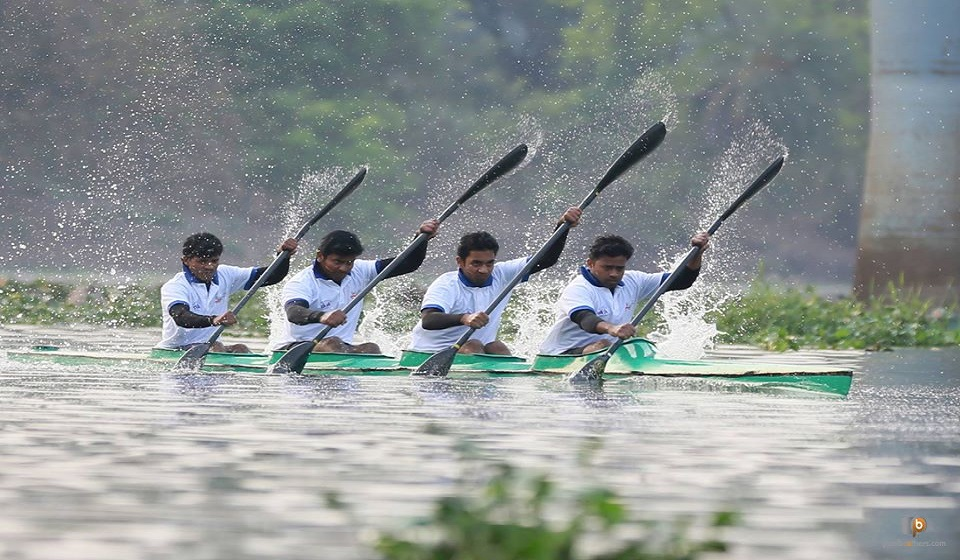
\includegraphics[width=0.7\linewidth]{Regatta649.jpg}
  \label{fig:3} 
\end{center}
\subsubsection{MindSpark}
MindSpark is the annual technical festival hosted by the college and established in 2007. The idea behind MindSpark originated from the need to unite various departmental level festivals that were scattered across the academic calendar. It features about 50 events across various disciplines of engineering and has been backed by the support of industrial sponsors who also associate with COEP for placement. This event is usually scheduled in an odd semester (around September) and is of 3 days (usually weekend)
\begin{center}
  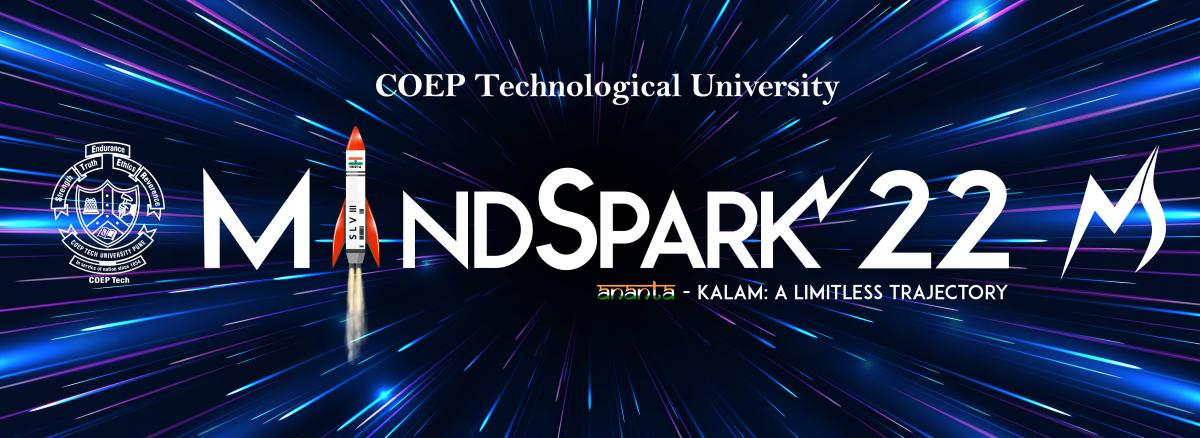
\includegraphics[width=0.7\linewidth]{MindSpark.jpg}
  \label{fig:4} 
\end{center}
\subsubsection{Impressions}
Impressions, is the annual cultural festival of CoEP, which is held every year in the 2nd week of December and lasts for 3 days. Impressions was formed as a platform "For the Artists, By the Artists", to provide opportunities for people from the fields of Dance, Music, Theater, Art, and Fashion to display their talent. The events span over six main modules, namely – Dance, Music, Arts and Crafts, Dramatics, Photography, and Writing.
\begin{center}
  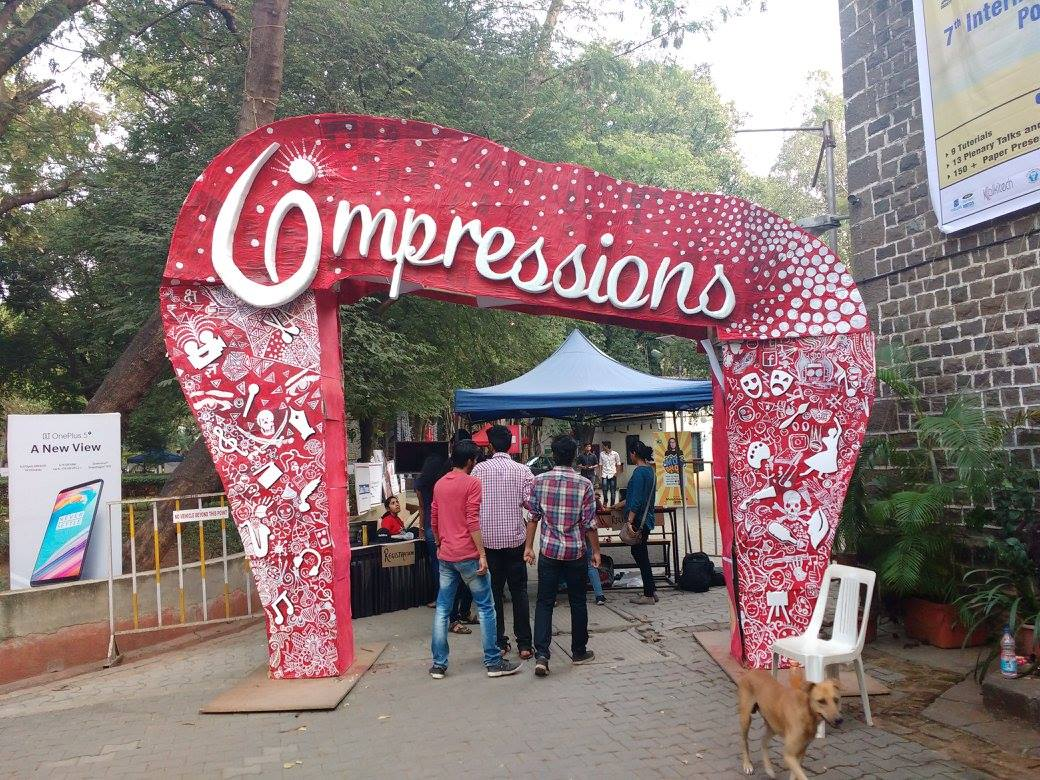
\includegraphics[width=0.5\linewidth]{impressions1.jpg}
  \label{fig:5} 
\end{center}
\subsection{Student Clubs and Chapters}
\subsubsection{CSI COEP Student Chapter}
The Computer Society of India (CSI) Student Chapter of College of Engineering Pune (COEP), established in October 2018 is the college's largest technical chapter. It organizes a number of technical activities including workshops, competitions, technical symposiums, guest lectures etc. for its student members. Under the guidance of Department of Computer Engineering and Information Technology COEP, the student chapter has over 300 members and is run by a Core Team and faculty from the department

\subsubsection{Team Nemesis Racing (Baja SAE)}
COEP won overall championship at BAJA 2017 competition creating a hat trick of records. In the 10th edition of Mahindra BAJA, a total of 415 entries applied for the event from 185 colleges that participated at a virtual stage, out of which 150 teams were selected for m- BAJA, while 35 teams for eBAJA. In the final round or the endurance test, 118 teams participated in the competition which was held from 16 to 21 February 2017 at the NATRIP facility in Pithampur, Indore. Out of the 12 award categories, COEP won 7 awards in BAJA competition 2017 retaining the Overall Championship

\subsubsection{COEP robotics team}
COEP Robotics Team is represented by the Robot Study Circle(RSC). The Club has industrial collaboration with Siemens PLM as a title sponsor,Pneumatics, Schmalz India, Pepperl Fuchs, and Robolab Technologies. Members of RSC are members of the first ever institute student chapter of THE ROBOTICS SOCIETY established in India at College of Engineering Pune
\subsubsection{Participation in Guinness World Records}
The college has made three entries so far in the Guinness World Record books. It holds the record for "Most people skipping on the same rope", which still stands as the world record and "The longest painting by numbers"and for "Most number of people solving the Rubik's cube"
\end{document}